\documentclass{standalone}
\usepackage{tikz}
\usetikzlibrary{patterns, positioning}


\begin{document}
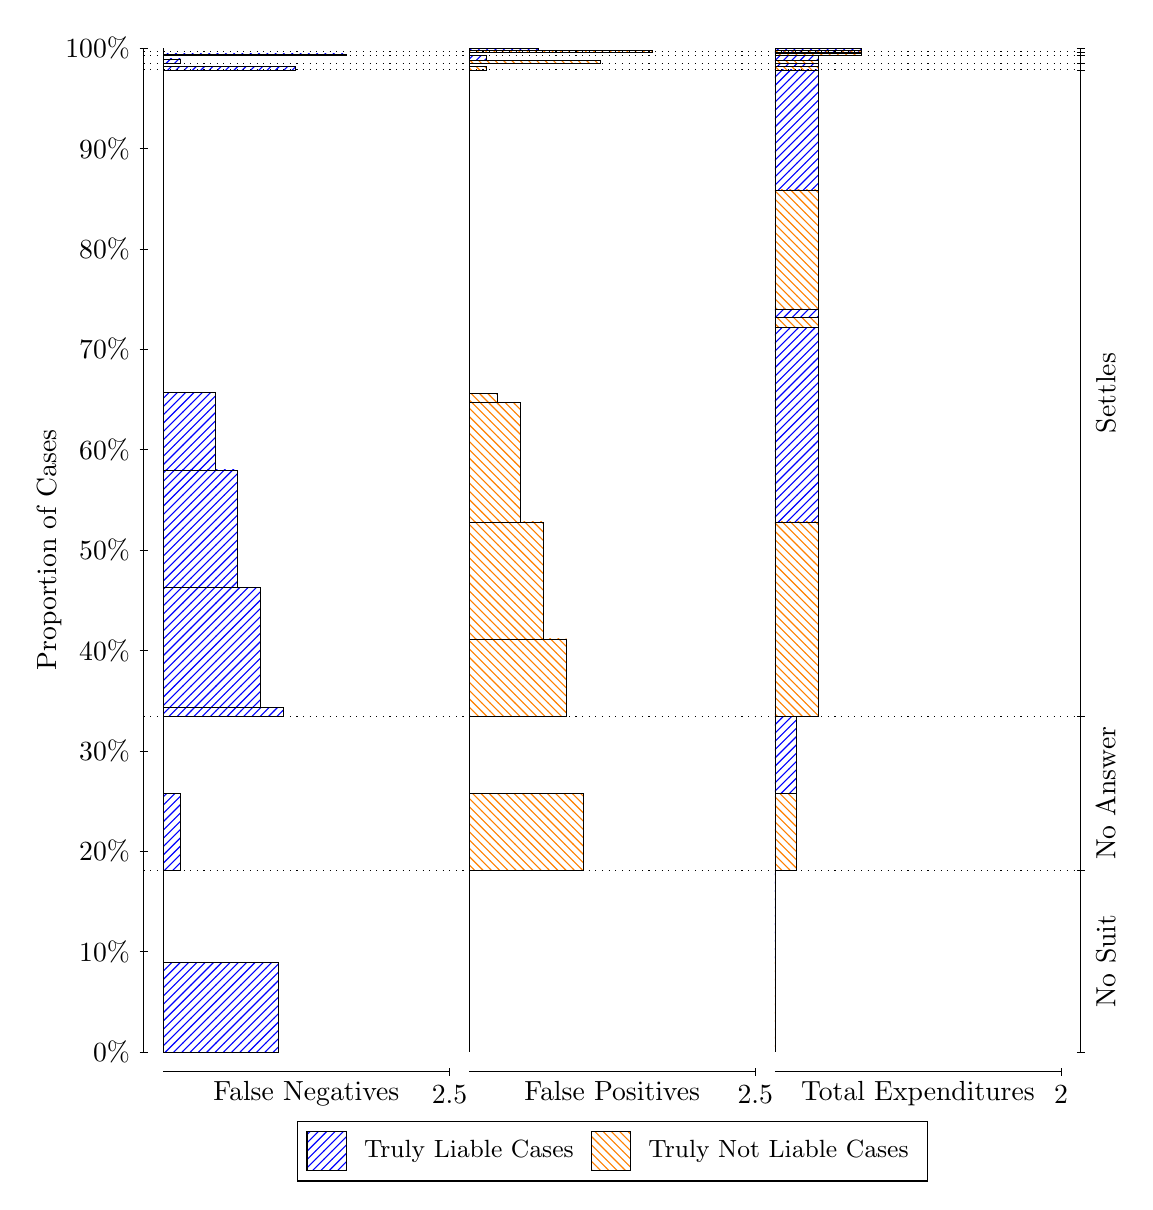
\begin{tikzpicture}
\draw[black, very thin] (1.5,1.75) -- (1.5,14.5);
\node[rotate=90, text=black, anchor=center] at (0.3, 8.125) {Proportion of Cases};
\draw[black, very thin] (1.45,1.75) -- (1.55,1.75);
\node[text=black, anchor=east] at (1.45, 1.75) {0\%};
\draw[black, very thin] (1.45,3.025) -- (1.55,3.025);
\node[text=black, anchor=east] at (1.45, 3.025) {10\%};
\draw[black, very thin] (1.45,4.3) -- (1.55,4.3);
\node[text=black, anchor=east] at (1.45, 4.3) {20\%};
\draw[black, very thin] (1.45,5.575) -- (1.55,5.575);
\node[text=black, anchor=east] at (1.45, 5.575) {30\%};
\draw[black, very thin] (1.45,6.85) -- (1.55,6.85);
\node[text=black, anchor=east] at (1.45, 6.85) {40\%};
\draw[black, very thin] (1.45,8.125) -- (1.55,8.125);
\node[text=black, anchor=east] at (1.45, 8.125) {50\%};
\draw[black, very thin] (1.45,9.4) -- (1.55,9.4);
\node[text=black, anchor=east] at (1.45, 9.4) {60\%};
\draw[black, very thin] (1.45,10.675) -- (1.55,10.675);
\node[text=black, anchor=east] at (1.45, 10.675) {70\%};
\draw[black, very thin] (1.45,11.95) -- (1.55,11.95);
\node[text=black, anchor=east] at (1.45, 11.95) {80\%};
\draw[black, very thin] (1.45,13.225) -- (1.55,13.225);
\node[text=black, anchor=east] at (1.45, 13.225) {90\%};
\draw[black, very thin] (1.45,14.5) -- (1.55,14.5);
\node[text=black, anchor=east] at (1.45, 14.5) {100\%};

\draw[black, very thin] (13.4,1.75) -- (13.4,14.5);
\draw[black, very thin] (13.35,1.75) -- (13.45,1.75);
\node[anchor=west] at (13.35, 1.75) {};
\draw[black, very thin] (13.35,4.0533) -- (13.45,4.0533);
\node[anchor=west] at (13.35, 4.0533) {};
\draw[black, very thin] (13.35,6.0148) -- (13.45,6.0148);
\node[anchor=west] at (13.35, 6.0148) {};
\draw[black, very thin] (13.35,14.223) -- (13.45,14.223);
\node[anchor=west] at (13.35, 14.223) {};
\draw[black, very thin] (13.35,14.303) -- (13.45,14.303);
\node[anchor=west] at (13.35, 14.303) {};
\draw[black, very thin] (13.35,14.402) -- (13.45,14.402);
\node[anchor=west] at (13.35, 14.402) {};
\draw[black, very thin] (13.35,14.451) -- (13.45,14.451);
\node[anchor=west] at (13.35, 14.451) {};
\draw[black, very thin] (13.35,14.5) -- (13.45,14.5);
\node[anchor=west] at (13.35, 14.5) {};

\draw[black, very thin, pattern color=blue, pattern=north east lines] (1.75,1.75) rectangle (3.2033,2.8841);
\draw[black, very thin, pattern color=orange, pattern=north west lines] (1.75,2.8841) rectangle (1.75,4.0533);
\draw[black, very thin, pattern color=blue, pattern=north east lines] (1.75,4.0533) rectangle (1.968,5.0341);
\draw[black, very thin, pattern color=orange, pattern=north west lines] (1.75,5.0341) rectangle (1.75,6.0148);
\draw[black, very thin, pattern color=blue, pattern=north east lines] (1.75,6.0148) rectangle (3.276,6.1244);
\draw[black, very thin, pattern color=blue, pattern=north east lines] (1.75,6.1244) rectangle (2.9853,7.6483);
\draw[black, very thin, pattern color=blue, pattern=north east lines] (1.75,7.6483) rectangle (2.6947,9.1422);
\draw[black, very thin, pattern color=blue, pattern=north east lines] (1.75,9.1422) rectangle (2.404,10.123);
\draw[black, very thin, pattern color=orange, pattern=north west lines] (1.75,10.123) rectangle (1.75,14.223);
\draw[black, very thin, pattern color=blue, pattern=north east lines] (1.75,14.223) rectangle (3.4213,14.263);
\draw[black, very thin, pattern color=orange, pattern=north west lines] (1.75,14.263) rectangle (1.75,14.303);
\draw[black, very thin, pattern color=blue, pattern=north east lines] (1.75,14.303) rectangle (1.968,14.363);
\draw[black, very thin, pattern color=orange, pattern=north west lines] (1.75,14.363) rectangle (1.75,14.402);
\draw[black, very thin, pattern color=blue, pattern=north east lines] (1.75,14.402) rectangle (4.0753,14.426);
\draw[black, very thin, pattern color=orange, pattern=north west lines] (1.75,14.426) rectangle (1.75,14.451);
\draw[black, very thin, pattern color=orange, pattern=north west lines] (1.75,14.451) rectangle (1.75,14.472);
\draw[black, very thin, pattern color=blue, pattern=north east lines] (1.75,14.472) rectangle (1.75,14.5);
\draw[black, very thin, pattern color=orange, pattern=north west lines] (5.6333,1.75) rectangle (5.6333,2.9192);
\draw[black, very thin, pattern color=blue, pattern=north east lines] (5.6333,2.9192) rectangle (5.6333,4.0533);
\draw[black, very thin, pattern color=orange, pattern=north west lines] (5.6333,4.0533) rectangle (7.0867,5.0341);
\draw[black, very thin, pattern color=blue, pattern=north east lines] (5.6333,5.0341) rectangle (5.6333,6.0148);
\draw[black, very thin, pattern color=orange, pattern=north west lines] (5.6333,6.0148) rectangle (6.8687,6.9956);
\draw[black, very thin, pattern color=orange, pattern=north west lines] (5.6333,6.9956) rectangle (6.578,8.4827);
\draw[black, very thin, pattern color=orange, pattern=north west lines] (5.6333,8.4827) rectangle (6.2873,9.9958);
\draw[black, very thin, pattern color=orange, pattern=north west lines] (5.6333,9.9958) rectangle (5.9967,10.115);
\draw[black, very thin, pattern color=blue, pattern=north east lines] (5.6333,10.115) rectangle (5.6333,14.223);
\draw[black, very thin, pattern color=orange, pattern=north west lines] (5.6333,14.223) rectangle (5.8513,14.262);
\draw[black, very thin, pattern color=blue, pattern=north east lines] (5.6333,14.262) rectangle (5.6333,14.303);
\draw[black, very thin, pattern color=orange, pattern=north west lines] (5.6333,14.303) rectangle (7.3047,14.343);
\draw[black, very thin, pattern color=blue, pattern=north east lines] (5.6333,14.343) rectangle (5.8513,14.402);
\draw[black, very thin, pattern color=orange, pattern=north west lines] (5.6333,14.402) rectangle (5.6333,14.427);
\draw[black, very thin, pattern color=blue, pattern=north east lines] (5.6333,14.427) rectangle (5.6333,14.451);
\draw[black, very thin, pattern color=orange, pattern=north west lines] (5.6333,14.451) rectangle (7.9587,14.472);
\draw[black, very thin, pattern color=blue, pattern=north east lines] (5.6333,14.472) rectangle (6.5053,14.5);
\draw[black, very thin, pattern color=orange, pattern=north west lines] (9.5167,1.75) rectangle (9.5167,2.9192);
\draw[black, very thin, pattern color=blue, pattern=north east lines] (9.5167,2.9192) rectangle (9.5167,4.0533);
\draw[black, very thin, pattern color=orange, pattern=north west lines] (9.5167,4.0533) rectangle (9.7892,5.0341);
\draw[black, very thin, pattern color=blue, pattern=north east lines] (9.5167,5.0341) rectangle (9.7892,6.0148);
\draw[black, very thin, pattern color=orange, pattern=north west lines] (9.5167,6.0148) rectangle (10.062,8.4827);
\draw[black, very thin, pattern color=blue, pattern=north east lines] (9.5167,8.4827) rectangle (10.062,10.957);
\draw[black, very thin, pattern color=orange, pattern=north west lines] (9.5167,10.957) rectangle (10.062,11.076);
\draw[black, very thin, pattern color=blue, pattern=north east lines] (9.5167,11.076) rectangle (10.062,11.186);
\draw[black, very thin, pattern color=orange, pattern=north west lines] (9.5167,11.186) rectangle (10.062,12.699);
\draw[black, very thin, pattern color=blue, pattern=north east lines] (9.5167,12.699) rectangle (10.062,14.223);
\draw[black, very thin, pattern color=orange, pattern=north west lines] (9.5167,14.223) rectangle (10.062,14.262);
\draw[black, very thin, pattern color=blue, pattern=north east lines] (9.5167,14.262) rectangle (10.062,14.303);
\draw[black, very thin, pattern color=orange, pattern=north west lines] (9.5167,14.303) rectangle (10.062,14.343);
\draw[black, very thin, pattern color=blue, pattern=north east lines] (9.5167,14.343) rectangle (10.062,14.402);
\draw[black, very thin, pattern color=orange, pattern=north west lines] (9.5167,14.402) rectangle (10.607,14.427);
\draw[black, very thin, pattern color=blue, pattern=north east lines] (9.5167,14.427) rectangle (10.607,14.451);
\draw[black, very thin, pattern color=orange, pattern=north west lines] (9.5167,14.451) rectangle (10.607,14.472);
\draw[black, very thin, pattern color=blue, pattern=north east lines] (9.5167,14.472) rectangle (10.607,14.5);
\draw[black, dotted] (1.5,4.0533) -- (13.4,4.0533);
\draw[black, dotted] (1.5,6.0148) -- (13.4,6.0148);
\draw[black, dotted] (1.5,14.223) -- (13.4,14.223);
\draw[black, dotted] (1.5,14.303) -- (13.4,14.303);
\draw[black, dotted] (1.5,14.402) -- (13.4,14.402);
\draw[black, dotted] (1.5,14.451) -- (13.4,14.451);
\draw[black, very thin] (1.75,1.5) -- (5.3833,1.5);
\node[text=black, anchor=north] at (3.5667, 1.5) {False Negatives};
\draw[black, very thin] (5.3833,1.45) -- (5.3833,1.55);
\node[text=black, anchor=north] at (5.3833, 1.45) {2.5};

\draw[black, very thin] (5.6333,1.5) -- (9.2667,1.5);
\node[text=black, anchor=north] at (7.45, 1.5) {False Positives};
\draw[black, very thin] (9.2667,1.45) -- (9.2667,1.55);
\node[text=black, anchor=north] at (9.2667, 1.45) {2.5};

\draw[black, very thin] (9.5167,1.5) -- (13.15,1.5);
\node[text=black, anchor=north] at (11.333, 1.5) {Total Expenditures};
\draw[black, very thin] (13.15,1.45) -- (13.15,1.55);
\node[text=black, anchor=north] at (13.15, 1.45) {2};

\node[text=black, centered, rotate=90] at (13.72, 2.9017) {No Suit};
\node[text=black, centered, rotate=90] at (13.72, 5.0341) {No Answer};
\node[text=black, centered, rotate=90] at (13.72, 10.119) {Settles};





\draw (7.449999999999999,1.5) node[draw=none] (baseCoordinate) {};
\begin{scope}[align=center]
        \matrix[scale=0.5, draw=black, below=0.5cm of baseCoordinate, nodes={draw}, column sep=0.1cm]{
            \node[rectangle, draw, minimum width=0.5cm, minimum height=0.5cm, pattern color=blue, pattern=north east lines] {}; &
            \node[draw=none, font=\small, text=black] (B) {Truly Liable Cases}; &
            \node[rectangle, draw, minimum width=0.5cm, minimum height=0.5cm, pattern color=orange, pattern=north west lines] {}; &
            \node[draw=none, font=\small, text=black] (B) {Truly Not Liable Cases}; \\
            };
\end{scope}

\end{tikzpicture}
\end{document}